\documentclass[11pt,a4paper]{article}
\usepackage[margin=25mm]{geometry}
\usepackage[T1]{fontenc}
\usepackage{lmodern}
\usepackage{amsmath,amssymb,graphicx,booktabs,tabularx,float,changepage,array,textcomp}
\usepackage{cite}
\usepackage[font=small,labelfont=bf,labelsep=period]{caption}
\usepackage{setspace,microtype,url}
\usepackage[hypertexnames=false]{hyperref}
\hypersetup{hidelinks,pdftitle={Experimental context limits transfer of microprotein sequence scores},pdfauthor={Robin Gounder and Samuel Schmidt},pdfkeywords={microproteins; noncanonical open reading frames; protein stability; sequence predictors; reporter assays; cross-assay transfer; reproducibility}}
\setstretch{1.10}
\setlength{\parskip}{3pt}
\setlength{\parindent}{1em}
\setlength{\emergencystretch}{3em}
\clubpenalty=10000\widowpenalty=10000
\pagestyle{plain}
\raggedbottom
\renewcommand{\topfraction}{.95}
\renewcommand{\bottomfraction}{.90}
\renewcommand{\textfraction}{.05}
\renewcommand{\floatpagefraction}{.80}
\setcounter{topnumber}{3}\setcounter{bottomnumber}{2}\setcounter{totalnumber}{5}

\renewcommand{\figurename}{Fig}
\graphicspath{{figures/}}
\title{Experimental context limits transfer of microprotein sequence scores}
\author{Robin Gounder\textsuperscript{1}, Samuel Schmidt\textsuperscript{2,3}\\[4pt]
\small\textsuperscript{1}University of Cambridge\\
\small\textsuperscript{2}Vaionex Corporation\\
\small\textsuperscript{3}Cornell University\\[4pt]
\small Correspondence: \href{mailto:robin@gounder.com}{robin@gounder.com}\\
\small Samuel Schmidt: \href{mailto:samuel@vaionex.com}{samuel@vaionex.com}}
\date{3 November 2026}
\begin{document}
\maketitle

\begin{abstract}
We asked whether microprotein sequence scores validated for one experimental
target remain useful after the assay, sequence input or decision changes.
Using published data, we distinguish a core reporter benchmark from
retrospective transfer extensions and exploratory diagnostics. Exact-sequence
joins, dependence-controlled evaluation and source-only training define the
comparisons. Among 1,072 development constructs, annotation-trained
composition resemblance correlated negatively with reporter accumulation
(Spearman $\rho=-0.292$), whereas outcome-trained composition and
terminal-aware models reached $0.747$ and $0.780$. Tests using 1,044 identical
peptides across reporter contexts, independent canonical tiles and 1,743
paired sequence changes showed that favorable within-context rankings did
not imply reliable transfer. Terminal features could improve within-context
prediction while reducing cross-context performance, and a model preferred
by global correlation was not always preferred for top-decile selection.
Source-population exclusions, matched inputs, training-exposure audits and
strong published baselines also changed the eligible comparisons and
narrowed apparent improvements. The practical implication is to validate a
score against the intended measurement, input and decision, and to test
paired effects before using a ranking model to prioritize edits. These
results define specific transfer boundaries rather than a universal
predictor. Native turnover and peptide-dependent activity remain separate
experimental questions.
\end{abstract}
\noindent\textbf{Keywords:} microproteins; noncanonical open reading frames; protein stability; sequence predictors; reporter assays; cross-assay transfer; reproducibility
\clearpage
\section{Introduction}
Microprotein sequence scores can address three different questions: whether
a sequence resembles an annotated protein, how much product accumulates in
a reporter assay, and how a sequence edit changes the measured outcome.
Performance on one question does not establish performance on the others.

Thousands of translated open reading frames fall outside conventional
protein annotations. Standardized catalogues support their study
\cite{mudge,chothani}, but translation, peptide accumulation and
peptide-dependent function require distinct evidence. Selected noncanonical
peptides already have motif-dependent cellular phenotypes and native
complex structures \cite{samandi,brownmitoribosome,rathoremief}.
Conversely, an upstream ORF can regulate downstream expression through its
RNA architecture or the act of translation \cite{shepelev}.
Endogenous variant/pathway tests and engineered degron-exposure experiments
provide further validation precedents \cite{ghosh,hasenjaeger}.

The six-feature XGBoost nORF Score showed no significant association with
EggNOG Gene Ontology annotation \cite{gounder}. Our controlled reanalysis
retained compositional differences after exact length matching.
We evaluate sequence representations
against measured reporter outcomes and sequence interventions.

Annotation and detection predictors have their own intended targets.
ShortStop prioritizes resemblance to curated microproteins relative to
synthetic references \cite{shortstop}. PepScore integrates ORF features and
was accompanied by individual expression assays \cite{yang}. Recent
preprints distinguish Ribo-supported from MS-supported prediction or model
repository MS detection using translation, conservation and peptide
attributes \cite{trans2ms,fierro}. Reporter transfer evaluates a different
endpoint; a faithful comparison must also retain any native RNA context
and other inputs required by the original model.

Composition-based degradation prediction and sequence-context effects have
established precedents. QCDPred predicts yeast quality-control degrons from
composition, with companion work testing human reporters
\cite{qcdpred,mashahreh}. Composition-only prediction also supports internal
degron mapping \cite{zhanginternal}. Guo et al. relate composition, genetic-code
and GC biases, disorder and terminal residues to reporter stability, including
substitutions, extensions and paired reporters \cite{guo}.
Cytosolic degron maps and terminal stability screens supply released PAP and
DEGRONOPEDIA baselines \cite{voutsinos,degronopedia,koren,timms}.
C-terminal sequence variation, composition-preserving shuffles and degradation
signatures have also been studied \cite{chu,casola}, with GC constraints as
established context \cite{roginski}.

Calibration and richer sequence representations likewise require comparison
with existing methods. Experiment-specific nonlinear calibration and variable
feature gains are documented \cite{schulze}. MAVE-NN and MoCHI model
genotype--phenotype and measurement relationships, with limits on identifying
their separate nonlinearities \cite{mavenn,mochi}. Joint abundance--binding
and abundance--activation models \cite{faureenergetic,leblancactivation},
and experimentally tested multi-mutant improvements \cite{gmma}, further
distinguish predictive fit from physical or functional interpretation.

The central question is when prediction validated in one context remains
useful in another. We first establish the core annotation-versus-reporter
comparison, then evaluate matched peptides across reporter contexts and
independent canonical-tile and paired-edit targets. Strong frozen baselines,
source-population rules and input/exposure controls bound those comparisons.
Secondary diagnostics and exploratory candidate links are retained in
S1 Text. The extensions are retrospective and outcome-informed; detailed
methods follow the main findings.

\section{Results}
The core reporter benchmark, central transfer extensions and exploratory
follow-up have different roles in the argument. All use existing data.
The later extensions are retrospective and outcome-informed; their central
narrative role does not make them preregistered or prospective confirmatory
tests. Detailed results, sensitivities and candidate-source audits are
retained in S1 Text.

\subsection{Core benchmark: training target determines reporter prediction}
On the 1,072 development constructs, the annotation-trained composition
resemblance score correlated negatively with the GFP--microprotein reporter
outcome ($\rho=-0.292$, 95\% conditional interval $-0.344$ to $-0.237$).
ShortStop's mean SAM probability had little monotonic association on its
covered set ($\rho=-0.018$; $n=1,057$). Models trained on the measured outcome
performed substantially better: composition model A reached $\rho=0.747$,
and terminal-aware T reached $0.780$ (Fig~\ref{fig:ranking};
Table~\ref{tab:native}). Useful composition prediction persisted in the
strict additional library ($\rho=0.719$).
These results distinguish annotation resemblance from this reporter
endpoint; they do not invalidate the original annotation task.

Adding native-order features to T gave a small primary rank increment,
$\Delta\rho=0.0040$ (95\% conditional interval $-0.0046$ to $0.0115$).
The increment varied across contexts. Coverage, dependence groups,
catalogue matching and all order sensitivities are reported in S1 Text
and Figs~S1--S3.
\begin{figure}[!htbp]
\centering
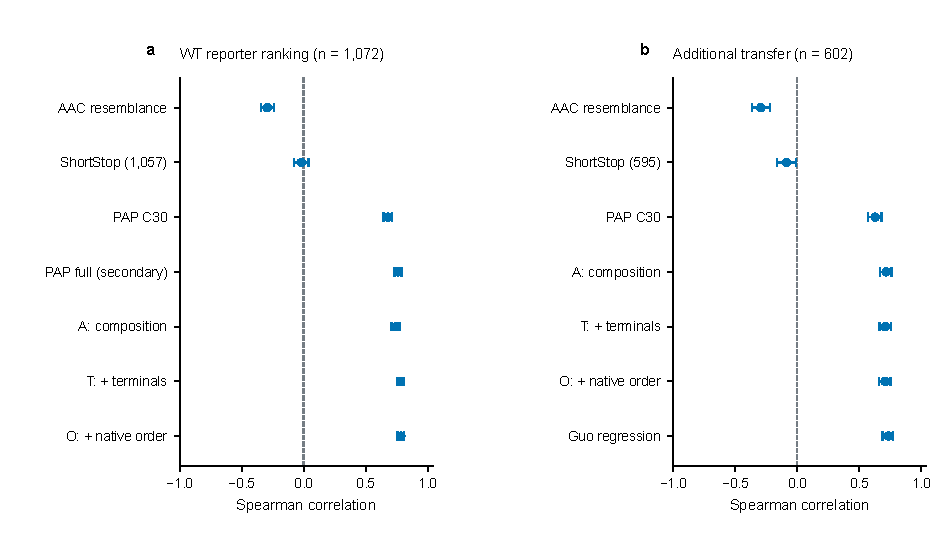
\includegraphics[width=\linewidth]{main/Fig1.pdf}
\caption{Reporter ranking and within-study transfer. Points show
Spearman correlation; bars show 95\% operational-group bootstrap intervals
conditional on fitted predictions. Raw annotation and PAP scores are ranking
comparators, not reporter probabilities. A/T/O are group-held-out in panel a and
trained on development WTs for transfer in panel b. Coverage exceptions are labelled.
The released Guo comparator is training-sequence/group-disjoint on these
additional cargos, but not demonstrably prospectively blinded.}
\label{fig:ranking}
\end{figure}
\begin{table}[H]\centering\small
\caption{Group-held-out native prediction and strict additional transfer.
MAE is shown only for direct endpoint models on reporter scale. Additional
sequences belong to the same publication, in a different library.}
\label{tab:native}
\begin{tabular}{lrrrr}\toprule
 & \multicolumn{2}{c}{GFP--MP WT, $n=1,072$} & \multicolumn{2}{c}{Additional strict, $n=602$}\\
Model & $\rho$ & MAE & $\rho$ & MAE\\\midrule
L: length & 0.207 & 0.2261 & 0.167 & 0.1743\\
A: composition & 0.747 & 0.1425 & 0.719 & 0.1259\\
T: plus terminals & 0.780 & 0.1362 & 0.712 & 0.1311\\
O: plus native order & 0.784 & 0.1354 & 0.710 & 0.1314\\
T plus shuffled order 1 & 0.770 & 0.1388 & 0.703 & 0.1344\\
T plus shuffled order 2 & 0.775 & 0.1380 & --- & ---\\
T plus shuffled order 3 & 0.771 & 0.1378 & --- & ---\\\bottomrule
\end{tabular}\end{table}

\subsection{Central retrospective transfer: the same peptides behave differently across contexts}
Matching 1,044 peptide identities fixes sequence-cohort composition in the
comparison of Guo reporter contexts \cite{guo}. Observed rank agreement was
$\rho=0.522$ between the original GFP--MP and MP--mCherry configurations,
compared with $0.867$ between the two GFP libraries (Fig~\ref{fig:pairedtransfer}).
Source-trained T reached $\rho=0.560$ on MP--mCherry, versus $0.742$ for
target-trained T; reverse transfer reached $0.566$ on GFP--MP, versus
$0.767$ for target-trained T (Table~\ref{tab:pairedcontext}).
Composition alone transferred better than T between the original reporter
configurations, reaching $0.663$ and $0.648$ in the two directions.

The added terminal information therefore improved some within-context
rankings without uniformly improving transfer. Reporter identity,
orientation, linker/tag architecture and library conditions co-vary, so
this comparison does not isolate their causal contributions. Target-supervised
calibration did not remove the target-scale error gaps and is adaptation,
not independent validation of a frozen model.
\begin{figure}[!htbp]
\centering
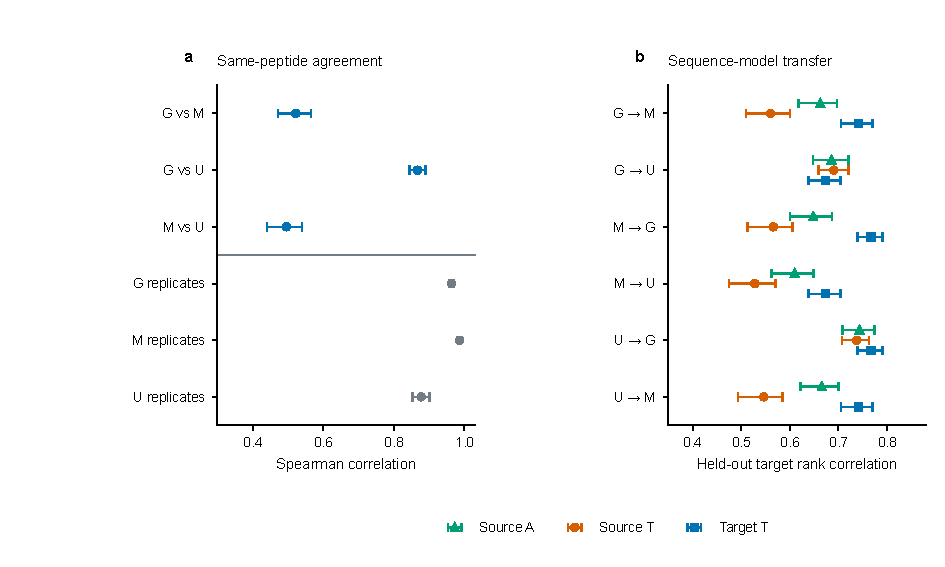
\includegraphics[width=\linewidth]{main/Fig2.pdf}
\caption{Same-peptide agreement and model transfer. a: correlations between context means and within-context biological
replicates on the common 1,044-peptide population; missing replicate pairs
are omitted as specified in the text. b: all six directed transfers of
source-trained A and T versus target-trained T on identical held-out groups.
Bars are descriptive 95\% operational-group bootstrap intervals conditional
on saved predictions. G: original GFP--MP; M: MP--mCherry;
U: mutagenesis-library GFP--MP. This is an exploratory same-study comparison.}
\label{fig:pairedtransfer}
\end{figure}
\begin{table}[H]\centering\small
\caption{Terminal-aware T transfer on the same 1,044 peptides.
G: original GFP--MP; M: MP--mCherry; U: mutagenesis-library GFP--MP.
Rank transfer uses the source model directly. MAE transfer uses target-scale
isotonic calibration learned entirely within outer training groups.
The target reference is trained on that target in the same group folds.}
\label{tab:pairedcontext}
\begin{tabular}{lrrrr}\toprule
 & \multicolumn{2}{c}{Target rank correlation} & \multicolumn{2}{c}{Target-scale MAE}\\
Transfer & Source-trained & Target-trained & Calibrated transfer & Target-trained\\\midrule
G to M & 0.560 & 0.742 & 0.2062 & 0.1572\\
G to U & 0.691 & 0.673 & 0.1211 & 0.1305\\
M to G & 0.566 & 0.767 & 0.1820 & 0.1401\\
M to U & 0.528 & 0.673 & 0.1492 & 0.1305\\
U to G & 0.737 & 0.767 & 0.1453 & 0.1401\\
U to M & 0.546 & 0.742 & 0.2065 & 0.1572\\
\bottomrule\end{tabular}\end{table}

\subsection{Central retrospective transfer: source and decision matter on independent cohorts}
Composition models trained in the two nORF reporter configurations reached
$\rho=0.816$ and $0.817$ on 14,143 eligible canonical tiles from 383 genes.
The corresponding T correlations were $0.812$ and $0.656$
(Fig~\ref{fig:external}; Table~\ref{tab:external}).
The GFP-source A-minus-T contrast was small and uncertain, whereas the
MP--mCherry-source gap was $0.161$ (95\% conditional interval $0.149$ to
$0.174$). This supports source-specific transfer behavior, not a general
claim that terminal features are harmful.

The decision metric also changed the comparison. GFP-trained T selected
higher-scoring top-decile tiles despite its slightly lower overall
correlation. Global rank association and prioritizing a subset are therefore
different evaluation targets. Frozen normalized QCDPred reached $\rho=0.800$,
narrowing the composition-head advantage; the top-decile selected-mean
difference intervals spanned zero.
\begin{table}[H]
\centering
\caption{Source-only nORF models evaluated on independent canonical tiles.
All rows use the same 14,143 held-out tiles from 383 gene groups. Selected
means are measured target-assay scores among the highest-scoring 1,415
tiles under each frozen policy; they are not source-scale predictions.}
\label{tab:external}
\small
\begin{tabular}{llrr}\toprule
Source training & Model & External $\rho$ & Selected assay mean\\\midrule
GFP--MP & A & 0.816 & 0.5976\\
GFP--MP & T & 0.812 & 0.6121\\
MP--mCherry & A & 0.817 & 0.5970\\
MP--mCherry & T & 0.656 & 0.5506\\\bottomrule
\end{tabular}
\end{table}
\begin{figure}[!htbp]
\centering
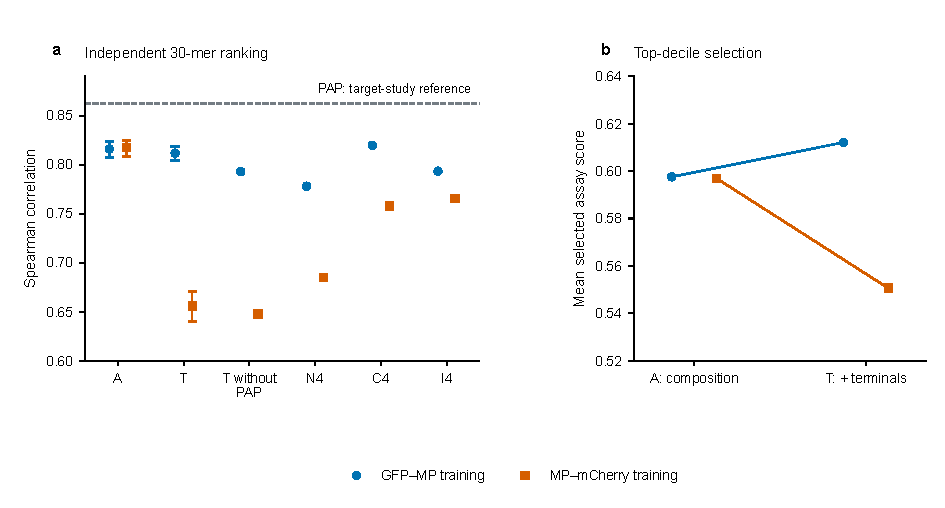
\includegraphics[width=\linewidth]{main/Fig3.pdf}
\caption{Source context and decision metric change the transfer comparison. a: independent-target Spearman correlation for both source-trained heads.
Intervals for A/T are conditional 95\% gene-bootstrap intervals; other
diagnostics are point estimates. The dashed PAP reference was trained in the
target study. N4/C4/I4 each add 80 positional columns to A; T without PAP
removes its pretrained components. b: mean measured target score among
each policy's highest-scoring 10\%; policy contrasts and uncertainty are
reported in the text and S9 Data. The source of the 30-mer assay is
independent; the target objects are canonical tiles rather than native nORFs.}
\label{fig:external}
\end{figure}

Independent paired changes supplied a separate intervention test. On the
1,743 matched 58-mer pairs retained after common source/PAP exclusions,
source-WT calibration improved linear full58 PAP from $\rho=0.651$ to
$0.692$. Raw published nonlinear PAP already reached $0.729$, and its
additional calibration gain was $0.006$ (95\% conditional interval
$-0.002$ to $0.014$; Fig~\ref{fig:published}; Table~\ref{tab:neural}).
Thus the specified linear improvement does not establish a general
calibration advance. PAP's author-held-out canonical-tile performance is
a target-study reference, not independent external validation of PAP.
\begin{figure}[!htbp]
\centering
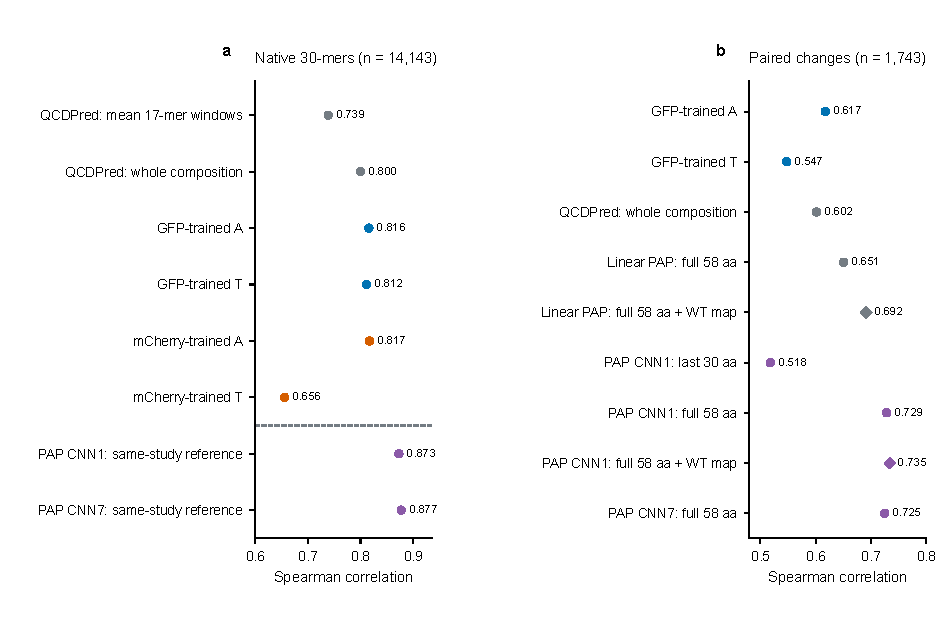
\includegraphics[width=\linewidth]{main/Fig4.pdf}
\caption{\textbf{Published baseline challenge across two fixed cohorts.}
(a) Native ranking on 14,143 tiles/383 genes. The dashed separator distinguishes
PAP neural models trained in that study from externally trained references.
(b) Paired RT-minus-WT ranking on 1,743 independent 58-mer window pairs/1,591
groups after common source/PAP-training exclusions. Diamonds denote Guo-WT-only
calibration. Full58 is supported variable-length inference beyond the training
30-mer length. Point estimates are shown; all variants, source contexts and
conditional paired contrasts are retained in S10 Data.}
\label{fig:published}
\end{figure}
\begin{table}[H]
\caption{\textbf{Independent paired-effect ranking for frozen baselines.}
All entries use the same 1,743 pairs. Calibration is learned solely from
Guo GFP--MP WTs. Full58 and C30 inputs are distinct prespecified representations.
Both endpoints of every pair are 58 residues. Values are Spearman correlations
with observed RT-minus-WT change; all components/sensitivities are in S10 Data.}
\label{tab:neural}
\centering\small
\begin{tabular}{lrr}
\toprule
Model and input & Raw & Source-WT calibrated\\
\midrule
QCDPred normalized & 0.602 & 0.622\\
Human25 normalized & 0.662 & 0.655\\
Linear PAP, C30 & 0.480 & 0.510\\
Linear PAP, full58 & 0.651 & 0.692\\
PAP CNN1, C30 & 0.518 & 0.530\\
PAP CNN1, full58 & 0.729 & 0.735\\
PAP CNN7, C30 & 0.524 & 0.533\\
PAP CNN7, full58 & 0.725 & 0.725\\
\bottomrule
\end{tabular}
\end{table}

\subsection{Retrospective controls: population, inputs and exposure bound the comparisons}
Eligibility rules changed an apparent feature advantage without changing
the predictions. On all 1,014 valid Leu-to-Ala pairs, T exceeded A by
$\Delta\rho=0.097$. Applying the original terminal-Leu exclusion left
798 pairs and a contrast of $-0.013$ (95\% conditional interval $-0.032$
to $0.005$). The append-edit advantage persisted. These are post-hoc
population contrasts using the source authors' rule \cite{guo}, not a
newly identified causal confound (Table~S1; S1 Text).

Input coverage also mattered. On the independent pairs, raw CNN1 reached
$\rho=0.518$ on C30 and $0.729$ on full58. The full58 representation
extrapolates beyond the training length, and this comparison does not
identify which residues or mechanisms explain the difference.

The terminal-model development-screen audit matched an endpoint in
1,454 of the 1,743 common-cohort pairs. Neither endpoint matched in
289 pairs. In that subset, DEGRONOPEDIA reached $\rho=0.537$, compared
with $0.521$ for PAP on identical C23 inputs and $0.761$ for full58 PAP
(Fig~\ref{fig:terminal}; Table~S2). The same-input difference interval
spanned zero. The audit does not recover individual training-split
membership or certify all historical exposure; its purpose is to bound
the eligible comparison.
\begin{figure}[!htbp]
\centering
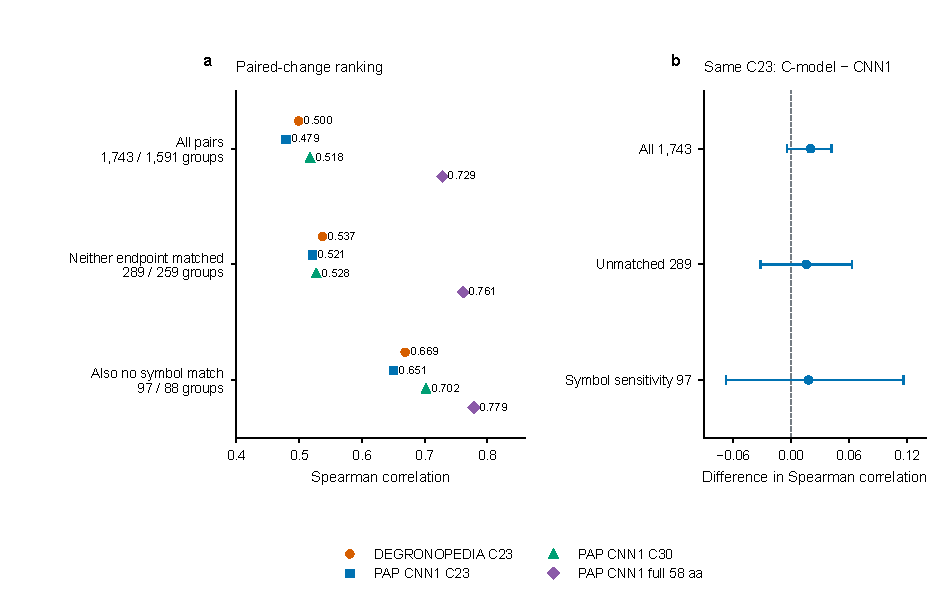
\includegraphics[width=\linewidth]{main/Fig5.pdf}
\caption{\textbf{Predictor exposure and matched-input controls bound model comparisons.}
(a) Paired-effect rank correlations for the C23 terminal model and PAP CNN1
using C23, C30 and full58 on three nested populations. The original
1,743-pair cohort excluded source/PAP training exposure, while 1,454 pairs
match an endpoint in the separate C23 development screen. Its actual
individual 90/10 split is unavailable. (b) C-model-minus-CNN1 contrasts
on identical C23 inputs, with 95\% conditional group-bootstrap intervals.
The matched-input controls are post hoc; all intervals span zero. The
97-pair available-symbol sensitivity is not alias-complete gene independence.
Different cohorts do not identify an exposure effect, and C23/full58 neural
inference extrapolates beyond the training length.}
\label{fig:terminal}
\end{figure}

\subsection{Exploratory challenges and candidate follow-up}
The separate, selected FLAG-expression panel retained a failed transfer:
primary MP--mCherry-trained T had $\rho=-0.652$ on the strict 20 constructs.
Selection, construct differences and the detection endpoint prevent a
population-wide failure estimate. All model/representation sensitivities,
within-study edit analyses and conditional-order controls remain available
in S1 Text and Figs~S3--S6.

Exact sequence joins also nominated three follow-up candidates:
RP11-620J15.3, JHDM1D-AS1 and the SLCO5A1 uORF peptide. Their existing
Leu-to-Ala and append measurements increased reporter output in both source
replicates, and the WT sequences have source interaction-tile annotations
\cite{guo,sandmann}. These exploratory links do not measure edited binding,
native turnover or peptide-dependent activity. The full 60-candidate roster,
source-positive/negative records, native-evidence reassessment and RNA-context
qualifications are retained in S1 Text and S12--S18 Data.

\section{Discussion}
\subsection{Transfer depends on the experimental question}
The central result is that microprotein sequence scores transfer according to
their training target, assay context and evaluation decision. Composition
distinguishes the defined reference populations and predicts reporter
accumulation when trained on that outcome. Annotation resemblance alone does
not provide a portable accumulation score. Terminal features, calibration and
residue order add predictive information in particular settings, without
establishing a universally preferred representation.

The evaluation population can change the conclusion even when predictions
remain fixed. The pooled terminal-feature advantage for Leu-to-Ala effects
disappears under the original source exclusion, whereas the append contrast
remains positive \cite{guo}. This limits generalization of the pooled result
without identifying a causal molecular explanation. The intended decision
also matters: GFP-trained T selects a higher-scoring top decile on canonical
tiles despite its slightly lower overall correlation. Ranking unmodified
peptides, selecting a subset and predicting an intervention are separate tests.

The matched-peptide analysis extends existing paired-reporter and
same-sequence context comparisons \cite{guo,larsen}. Fixing peptide identity
removes a sequence-cohort explanation, but reporter identity, orientation and
library conditions still co-vary; MP--mCherry also has a variable-length GS
linker and an HA tag. The comparison therefore measures transfer behavior
without isolating the responsible construct component. The selected
FLAG-expression panel adds an adverse transfer case, but its selection,
architecture and detection endpoint prevent a population-wide failure
estimate \cite{yang}.

\subsection{Input coverage and provenance shape predictor comparisons}
Strong published baselines materially narrow the calibration result.
Source-WT mapping improves linear PAP change prediction, but raw nonlinear
PAP performs better on the same independent pairs. The additional full58
neural-calibration interval spans zero, while the C30-to-full58 input change
has a much larger association with performance. Full58 inference extrapolates
beyond the training length, and this contrast does not identify a biological
cause. These comparisons make model architecture and input coverage essential
parts of evaluating a calibration claim.

Experiment-specific nonlinear readouts and separation of measurement from
latent biological maps are established methods \cite{schulze,mavenn,mochi}.
Physical interpretation requires additional anchors: Salinas and Ranganathan
used affinity-characterized mutants and WT-affinity corrections, while their
homologue comparison retained a hypothesized internal-equilibrium mechanism
\cite{salinas2018}. Joint folding/binding and abundance/activity models have
their own physical assumptions and validation targets
\cite{faureenergetic,leblancactivation}. Higher-order prediction and
domain-extension or ligand maps also use distinct proteins, substitutions
and validation settings \cite{architecture,pdzextensions,pdzcomparative}.
Our source-WT remapping has no independent molecular anchor and does not
recover an assay-independent physical stability scale.

Training exposure determines which model comparisons can be called
independent. The terminal-model audit restricts the eligible pairs, and
matched C23 inputs remove most of its apparent point-estimate gap against
CNN1. Intervals spanning zero demonstrate neither equivalence nor a universal
winner. Higher correlations after exclusions do not establish that exposure
caused inflation. Population and decision-metric effects have precedents
\cite{fawzy,gmma}; the added result is the specified shared-population
comparison with inspectable provenance. Likewise, the small property-feature
increment cannot be generalized to all order-aware models. CNN7 retains an
order increment on its source study's held-out tiles, while independent
paired-effect intervals span zero. Model shuffles test conditional predictive
information, not the biological effects of physically shuffling a peptide.

\subsection{Reporter prediction and native function require different evidence}
Sequence descriptors alone do not identify a degradation mechanism.
Composition-conditioned motif prioritization, degron scrambles and stabilized
full-length products already have experimental precedents
\cite{zhanginternal,mashahreh,chu}. Terminal screens distinguish encoded
sequence from exposed ends and pathway dependence from total stabilization
\cite{koren,timms}. Recognition, ubiquitination and proteasomal engagement are
distinct stages \cite{tripartite}, potentially affected by accessibility and
partner occupancy \cite{hasenjaeger,guharoymasking}. Steady-state accumulation
also depends on production: under a simple first-order balance,
$P_{\mathrm{ss}}=s/k$, where $s$ is production and $k$ includes degradation
and dilution. Production and turnover measurements are therefore needed for
a candidate-specific stability mechanism.

Annotation, detection and evolutionary origin address further distinct
targets \cite{shortstop,trans2ms,fierro,middendorf,roginski,cardiacevolution,vakirlis}.
A peptide-only reporter test cannot refute a model requiring unavailable
native RNA context. HLA presentation, intact-product accumulation and
peptide-dependent function also require different evidence
\cite{wacholder,deutsch}; missing detection or screen records are not
established functional negatives.

The three candidate links define experiments rather than complete them.
Synthetic-peptide interactions need not reproduce native stability,
concentration or compartmentalization \cite{sandmann}, and the edited
products were not tested for binding or activity. Characterized MIEF1-MP70
and MRPL33\_65 controls have native structural evidence
\cite{brownmitoribosome}, but neither has an exact primary GFP/edit pair in
our bridge. Selected rescue and assembly studies establish functional
noncanonical products \cite{chenfunctional,prensner,hofman,samandi,rathoremief},
while abundance and functional readouts can diverge \cite{salghetti,matreyek}.
JHDM1D-AS1/DHX15 and RP11-620J15.3 RNA studies do not isolate the nominated
peptides \cite{yao,malmstrom,liu}; the reported DHX15 turnover assay measures
DHX15 rather than JHDM1D-AS1 peptide clearance. RNA architecture, translation and
released-peptide activity require candidate-appropriate controls
\cite{yang,shepelev,devaux}.

\subsection{Practical implications}
For reporter accumulation, choose or validate a score against the actual
measurement and construct context; annotation resemblance or detection
probability is not an interchangeable endpoint.

For cross-study comparisons, retain the input sequence seen by each model,
audit training exposure and compare strong frozen baselines on a common
eligible population. Report coverage and the intended decision metric
alongside global correlation.

For edit prioritization, evaluate paired changes in the relevant sequence
population. Increased reporter output does not establish slower native
clearance or preserved activity; those require product-compatible
production, turnover and functional measurements.

\subsection{Limitations and next experiments}
Several extensions were retrospective and outcome-informed. We use aggregate
assay releases, operational dependence groups and intervals conditional on
fitted models, rather than raw-data reconstruction, exhaustive remote-homology
control or full retraining. Historical training snapshots are incomplete,
and post-hoc intervals are not multiplicity-adjusted discovery tests.
Canonical tiles independently test our source-trained heads, but their
PAP-development provenance prevents treating the accompanying PAP scores
as independent validation of PAP. The three-row paper/release discrepancy
is recorded. The common paired cohort audits source/PAP genes and windows,
without certifying independence for every predictor. The terminal-model
audit lacks individual split membership, does not resolve every alias or
remote homologue, and does not audit N-terminal exposure. Comparisons must
retain these coverage and provenance limits. The claim-focused literature
assessment does not establish exhaustive priority.

Native validation should first identify the intact or processed product
with an edit-compatible measurement and distinguish production from
clearance. WT, the individual edits and the unmeasured combined edit/append
panel should be tested separately. Binding or activity should be compared
across overlapping measured protein amounts, with a predefined equivalence
criterion for preservation. RNA, translation and recoded-peptide rescue
controls should separate transcript, translation-process and peptide-sequence
explanations. A masking hypothesis additionally requires a validated partner
perturbation and a clearance measurement. These experiments could establish
a candidate-specific biological relationship; the present work supplies
their nomination and the measured prediction-transfer limits.

\section{Conclusions}
Microprotein sequence scores should be validated for the measurement and
decision they will support. Composition transfers usefully in several
reporter settings, while gains from terminal features, calibration and
residue order depend on the source, input and endpoint. Strong published
baselines, matched inputs and predictor-specific exposure controls are
therefore necessary to interpret an apparent improvement. Exact candidate
links nominate native experiments that test production, clearance,
interaction and activity separately. The contribution is a reproducible
empirical account of these transfer boundaries; native peptide-dependent
function remains to be measured for the proposed edits.

\section{Materials and methods}
\subsection{Analysis hierarchy}
The core benchmark comprises the original dependence-controlled reporter
evaluation. We distinguish it from the later same-peptide, canonical-tile
and independent paired-effect transfer extensions. Those extensions are
central to the present scientific question but retrospective and informed
by earlier results. Source-population exclusions, input/exposure challenges,
order/calibration sensitivities, the selected FLAG panel and candidate joins
are explicitly secondary or exploratory. These labels describe analysis
roles, not preregistration or prospective confirmatory status. All outcomes,
including adverse transfer cases, remain reported in S1 Text.


\subsection{Controlled catalogue context and clustering reproduction}
The controlled catalogue analysis reconstructed 28,359 TransCODE Phase 2
candidates against hg38, audited current GENCODE v50 coding overlap and
retained 27,670 eligible nORFs. Canonical representatives were the longest
valid translated isoform per gene (19,563 genes). The protr descriptor
definitions were versioned \cite{xiao}. Default lag/lambda 30 restricted the
all-family comparison to proteins of at least 31 residues; no missing
long-lag features were imputed. Exact full-protein length matching after
dependence filtering yielded 744 comprehensive pairs, 245 Primary pairs and
472 pairs with an additional absolute GC caliper of 0.02. Matched pairs and
linked sequence/gene groups stayed in the same evaluation fold.

Clustering used the 1,488 comprehensive matched sequences, all 1,440
descriptors, equal-feature or equal-family weighting, PCA retaining 50
components, $k=2,3,5,8$, multiple seeds and 80\% subsampling. Native sequences
were compared with composition-preserving shuffles. A separate computational
rerun checked saved PCA memberships and two t-SNE maps. This reproduces the
controlled computation; the original cluster memberships remain unresolved. UMAP was not
rerun. The original matrix and complete historical settings remain unavailable.

\subsection{Experimental sources and target definitions}
Guo supplementary tables supply normalized fusion-reporter scores
\cite{guo}. The primary development set comprises 1,072 valid wild-type (WT)
GFP--microprotein (GFP--MP) cargos; 1,071 have both reported biological
replicates. The opposite MP--mCherry orientation supplies 1,046 measured WTs.
A separate GFP--MP mutagenesis library contains 1,072 WT baselines, 730
HLA-associated and 71 digest-MS-associated natural sequences, and engineered
variants. The additional 801 sequences are absent as exact peptides from the
released 1,072-row Guo regression-training table. They remain within the same
study, and their availability does not establish prospective blinding of the
published models.

We used released means, available biological replicate cells, oligos and
source-code metadata. The publisher's article-plus-supplement file subsequently
provided full STAR Methods access \cite{guo}. The source describes within-bin
counts-per-million normalization, five bin weights (0.1, 0.3, 0.5, 0.7, 0.9),
their counts-weighted average and replicate-specific min--max scaling.
We did not rerun that raw read processing or infer censoring from aggregate
scores. Raw read-depth and censoring information were not obtained for this
reanalysis. These limitations constrain error and detection interpretation.
Throughout, ``reporter score'' denotes the supplied assay measurement, not an
endogenous half-life, thermodynamic folding stability or function.

Exact sequence editing verified 1,014 global Leu-to-Ala pairs and 1,007
extensions by the constant C-terminal sequence DNYNEPKANQ. Observed change
was mutant minus WT score in the \textbf{same mutagenesis library}. Original and
mutagenesis-library WT measurements differ, so the former were not substituted
as mutant baselines. Missing outcomes or predictors were not replaced by zero.
These all-sequence-valid populations are broader than the source's specified
Leu-to-Ala analysis: its STAR Methods exclude WTs containing Leu at either
of the last two residues, and Fig. 4F states this restriction for the
WT/substitution/extension comparison \cite{guo}. After recovering the full
methods, we applied that WT-sequence rule to both edit families as a
post-hoc sensitivity, retaining all earlier fits and predictions. This
retained 798 Leu-to-Ala pairs in 611 operational groups and 802 append pairs
in 623 groups. All, retained and omitted strata, mean and both replicate
effects, all 20 original predictors and compatible-scale errors are supplied
in S12 Data. T-minus-A, O-minus-T and calibrated-minus-raw full-PAP rank
contrasts use 1,000 group resamples conditional on the original fits, with
no multiplicity adjustment. An independent workbook reader checked all
2,021 membership flags; an independent rank implementation checked 360 point
metrics and 18 point contrasts. Bootstrap distributions were not independently
replayed. This changes the evaluation population, not the fitted models,
and does not reproduce every original assay-processing decision.

The separate Yang assay contains 29 uORFs and eight other ORFs, with native
lengths 17--129 residues \cite{yang}. We translated all 37 supplied synthesized
constructs, verified their reported lengths and terminal DYKDDDDK FLAG tags,
and joined measurements by ORF name. Untreated outcomes are the mean of five
replicates for the 29 uORFs and four for the other eight. The target is
GFP-normalized FLAG-positive cell fraction, not the Guo numerical scale.
The source describes the 29 uORFs as randomly selected across PepScores;
the eight other ORFs were chosen with high scores. The combined 37-construct
set mixes these selection schemes and ORF classes; it is not a population-wide
validation sample.

\subsection{Dependence audit and score provenance}
Exact peptide identity, parental construct, available gene identities and
catalogue overlap groups supplied dependence links. Engineered sequences
shared by different parents connected those parents. We exhaustively aligned
eligible pairs among native assay peptides, Yang natives, annotation-reference
sequences and available ShortStop positive-reference counterparts. Local
Smith--Waterman alignment used BLOSUM62, gap-open 10 and gap-extension 1.
Primary edges required at least 60\% identity over alignment columns and at
least 80\% coverage of \textbf{both} full sequences; a 40\% identity graph was a
declared sensitivity. Length and composition bounds only removed pairs that
could not meet these criteria. Connected components defined split groups.
These are operational dependence groups, not proof of no remote homology or
pretraining exposure.

The annotation-trained AAC classifier retained the original fixed Extra Trees
configuration: 200 trees, maximum depth 10, minimum leaf 10, square-root
feature sampling, balanced classes and seed 100. Whole reference pairs and
linked reference split groups were removed to a fixed point if connected to
any Guo or Yang parent. Seeds 101 and 102 were sensitivity analyses. Higher
scores indicate canonical resemblance, opposite to the nORF Score convention \cite{gounder};
this classifier never fitted reporter outcomes.

ShortStop v1.2.0 (28 October 2026) precomputed scores were joined only after
independent GTF translation against hg38 verified exact peptide identity.
The primary continuous score was mean SAM probability across released models.
Published standard and stringent consensus calls were retained as distinct
threshold analyses. Actual supervised-positive identifiers were distinguished
from ToBePredicted records, which the inspected training code excludes from
supervision. The available 1,571 positive counterparts are current reviewed
sequences, not a complete historical training-sequence archive. Thus absence
of exact matches does not establish complete training or pretraining separation.

The frozen PAP human30 model was reimplemented from safely parsed published
numeric coefficients \cite{voutsinos}. Primary transfer uses the final
$\min(30,L)$ residues. Composition terms scale residue counts to 30 positions;
terminal, pair and triplet terms follow the released positional definition.
The full-peptide normalized-composition version is a secondary transfer, not
a newly fitted PAP model. Deposited Guo classification/regression predictions
were evaluated only on the additional natural sequences and their strict
subset, not against other methods' held-out predictions on Guo's own training
rows. Supplied PepScore values were used only for the exact Yang constructs;
missing transcript, domain or evolutionary covariates were not invented.

\subsection{Endpoint models, order controls and nested validation}
Models used five outer and three inner group folds. Groups were randomly
tie-broken with seed 20261031, sorted by descending size and greedily assigned
to the smallest fold without using outcomes. Ridge penalties
$\{0.1,1,10,100,1000\}$ were selected by inner mean absolute error (MAE).
Standardization and intercept fitting used each training split only.
All representations shared the same outer folds. Predictions and fit receipts
were saved for every held-out row.

The length model L contains log length and its square. A adds all 20 AAC
frequencies. T adds first-five and last-five residue one-hot encodings,
whole/N10/C10 hydropathy and PAP composition/terminal components. O adds 40
short-range property-product averages: eight default Moreau--Broto AAindex
properties at lags 1--5, standardized across amino acids, then centered and
scaled against 199 within-peptide shuffles. Shuffles preserve exact composition
and the first and last five residues. Zero null variance produces a zero
residual. This avoids lag-30 imputation and supplies features for short cargos.

Three independent shuffled-order representations add the same 40 standardized
features to T using additional shuffled realizations. They test representation
effects conditional on composition and terminal residues; the shuffled
peptides have no measured outcomes and are not labelled experimental negatives.
Raw order features, two extra fold seeds, 40\% identity grouping and fixed
Extra Trees regression for A/T/O were declared sensitivities. The tree
regressors used 200 trees, depth 10, leaf minimum 10 and feature fraction 0.7.
No outer-fold winner was substituted for the primary Ridge analysis.

Primary contrasts are O-minus-T rank correlation and T-minus-O MAE, with
1,000 operational-group bootstrap resamples conditional on saved predictions.
These intervals do not include full model-retraining uncertainty. Additional
intervals and subgroup results are descriptive; no secondary significance
claims or multiplicity-adjusted discovery list is made. No equivalence test
was performed. Median absolute biological-replicate disagreement and half
that value provide descriptive scale context, not a formal noise floor or
biological relevance threshold.

\subsection{Calibration, perturbation prediction and independent transfer}
Frozen scores were mapped to reporter scale using isotonic regression fitted
to training WTs within each group fold. Direction was determined by training
correlation and recorded, including reversed AAC-resemblance maps. Raw score
MAE was not compared across incompatible scales. For mutations, each parent's
WT and variant were predicted with the \textbf{same parent-held-out} model or
isotonic map trained on mutagenesis-library WTs. We report raw rank differences
as well as calibrated prediction changes. Zero change and an out-of-group
training-family mean are error baselines. Replicate-specific outcome changes
were analyzed separately.

Secondary mutation-trained Ridge models use mutant-minus-WT changes in A/T/O
features and grouped nested evaluation within each family. Opposite-family
transfer trains on the other edit family after excluding all held-out parent
groups. This distinguishes native-score extrapolation, learning an edit
family, and transfer between edit families.

Before scoring Yang outcomes, main predictions and model choices were saved
in a validation-release receipt. Primary direct transfer trained on MP--mCherry
WTs, whose cargo has a free N terminus and masked C terminus, as an approximate
context choice for a C-terminal FLAG construct. Actual FLAG-fusion sequence
features were primary; native-only features and GFP--MP training were declared
sensitivities. Every training group connected to any Yang construct was removed
from these direct-model fits. We did not fit, invert, calibrate or select models
on the Yang outcomes. The representation is still a cargo approximation: neither
Guo carrier architecture is identical to a FLAG construct. Analyses report all
37, the 27 without exact Guo overlap, and the 20 passing strict separation from
all retrieved Guo natural cohorts. Rank correlation and AUROC at the authors'
5\% expression threshold are reported; cross-assay absolute MAE is suppressed.


\subsection{Exploratory paired reporter-context analysis}
To compare contexts on the same peptide population, we joined WT records by
both source identifier and exact native amino acid sequence across original
GFP--MP (G), original MP--mCherry (M), and mutagenesis-library GFP--MP (U).
The complete-mean intersection contains 1,044 peptides in 783 primary
dependence groups. Of 1,072 G, 1,046 measured M and 1,072 U records, respectively
28, two and 28 fall outside this intersection. Biological-replicate agreement
was computed on available replicate pairs within this same population.
The extension was specified after inspecting aggregate paired correlations;
it is exploratory and does not supply independent-study validation.

All six directed transfers used the previously defined A and T representations
and nested Ridge settings, with identical five-fold assignments across the
three contexts. This common-cohort split differs from the earlier
1,072-row development split. Every model excluded the test peptide's entire dependence
group across contexts. The target-trained reference used target measurements
from the training groups; the source-trained model used source measurements
from those groups and was evaluated against the held-out target ranking.
For target-scale error, isotonic calibration used source predictions generated
by a further group cross-fit within each outer training partition,
paired with training-target measurements. Its monotonic direction was learned
there. Neither source fitting nor calibration used outer-test target outcomes.

A separate measured-source bridge fitted an isotonic map from paired
training measurements and required the test peptide's measured source score;
it is not a sequence-only method. Training-target means supplied an MAE
baseline. We repeated the sequence analysis with the prior 40\% identity
graph and split seed 20261032. Descriptive intervals use 1,000 group-bootstrap
resamples conditional on saved predictions, including paired contrasts on
identical target rows. No multiplicity-adjusted discoveries are claimed.

\subsection{Independent canonical-peptide transfer extension}
After examining the paired-context results, we specified a new comparison
before evaluating predictions against an independent target. We used the
author-held-out cytosolic 30-mer library from Voutsinos et al. \cite{voutsinos},
pinning the repository at commit
\texttt{9b3eafa6bd9730c558cd018063fa0180edf9db1a}.
The released split and original processing log both contain 15,818 test
members, whereas the paper states 15,815. We retained all valid released
members before exclusions and report this discrepancy. Exact author-training
peptide duplicates were absent. Excluding genes shared with the retrieved
Guo/annotation inputs and peptide matches at $\geq60\%$ identity and
$\geq80\%$ coverage of both sequences left 14,143 tiles from 383 ENSG
gene groups. The $40\%$ identity sensitivity retained 13,730 tiles. These
operational rules do not guarantee absence of remote homology.

A and T heads were fitted separately to the original 1,072 GFP--MP and
1,046 MP--mCherry WTs, using the benchmark's source-group tuning and
training-only scaling. All target predictions and input/model hashes were
frozen before joining released abundance scores. Target outcomes did not
select the source, sign, penalty or representation. A/T source features were
independently reconstructed and matched the saved benchmark exactly. We
report Spearman correlation and paired A-minus-T contrasts, with 1,000
gene-cluster bootstrap resamples conditional on fitted predictions. A second
source-only tuning seed is a sensitivity analysis; target-scale error was
not compared across these different assays.

Secondary diagnostics remove PAP from T or add 80 one-hot columns to A
for positions 2--5 (N4), the last four residues (C4), or the four central
residues (I4, zero-based slice $L//2-2:L//2+2$). Equal nominal dimension
does not equalize effective complexity or isolate terminal exposure. Source
grouped nested-CV results accompany these diagnostics. PAP internal/full
scores are target-study-trained held-out references, not equally external
competitors; their coefficients also contribute to T's pretrained features.

After initial transfer inspection, a secondary policy comparison reused the
earlier benchmark's $10\%$ selection fraction without target optimization.
Each frozen score selected its highest-ranked $\lceil0.1n\rceil$ tiles;
ties followed lexical peptide order. We report mean measured assay score
among selections and paired policy contrasts, recalculating selection in
each gene-bootstrap draw. This is retrospective assay-rank prioritization,
not prospective candidate or functional validation (S9 Data).

\subsection{Frozen published baselines and independent paired changes}
After the canonical-tile analysis, we added two secondary challenges with
protocols and prediction hashes recorded before their new model--outcome
associations. Earlier target results were already known. The original
QCDPred code and labeled training tiles were pinned to the authors' repository
commit \texttt{85979b1b4123b6b5391b617d16551969eda9f56e}
\cite{qcdpred}. We retained both the mean stability over complete overlapping
17-mers and a whole-cargo composition representation. The latter rescales
the sum of residue coefficients by $17/L$ before the published logistic
transform; it is a declared alternative representation, not the ordinary
17-mer-window output. No labeled training 17-mer exactly matched the tested
windows. This check is not an exhaustive homology certificate. The human25
composition model was retained with first-25 and whole-cargo normalization;
its native-tile results are target-study-trained references (S10 Data).

Chu Supplementary Data 1 contains 3,249 matched pairs \cite{chu}.
Both measured cargos have 58 residues. The RT-derived cargo comprises a
retained WT suffix followed by the readthrough sequence; 339 rows retain no
WT residues. These are terminal-window replacements, not simple appends to
the measured WT58. We required unique gene mapping, standard nonidentical
58/58 sequences, consistent reported sequence/length fields, and at least
60 reads at both endpoints in both replicates. Six Excel-date gene-name
artifacts were resolved by transcript/sequence mapping; two inconsistent
WT/shared-suffix rows were excluded rather than repaired from outcomes.
RT-minus-WT replicate means were checked against all released mean/delta
columns. Source gene and sequence exclusions used the preceding $60\%$
identity/$80\%$ bilateral-coverage rule, with $40\%$ sensitivity. The common
primary cohort additionally excluded PAP-training-linked genes and exact
PAP30/human25 training windows from either endpoint. This retained 1,743
pairs in 1,591 operational dependence groups joining gene identity and
identical endpoint sequences. The stricter cohort contains 1,738 pairs;
the source-head-only sensitivity contains 2,326. Current-transcript terminal
matching is an additional sensitivity, not outcome-based membership.

We froze A/T predictions fitted in each original Guo context, linear PAP
composition/terminal decompositions, QCDPred and human25. For every frozen
baseline, an increasing isotonic map used only the original 1,072 Guo GFP--MP
WT outcomes; calibrated changes subtract mapped endpoint scores. No Chu
outcome fitted or selected a source, direction, model or calibration. We
retained all 22 original raw/calibrated score variants, clipping and zero
mapped effects. Absolute errors on incompatible raw score scales are not
compared (S10 Data).

\subsection{Published neural PAP challenge and conditional order controls}
We then challenged these results with published default CNN1 and released
kernel-seven CNN7 PAP weights from the pinned Voutsinos release
\cite{voutsinos}. Other models' outcomes were already inspected, making this
a secondary stronger-baseline challenge. The internal channel applies a
kernel-one or kernel-seven convolution, global averaging and nonlinear dense
layers; a separate nonlinear channel encodes the final five residues.
The two channel scores are added. Original model classes and numeric HDF5
weights were used, adapting the Keras backend import and legacy layer loading
only. Independent NumPy forward passes verified the preserved graph and
weights. CNN1's internal channel is a nonlinear function of composition;
CNN7 can retain local order. Differences between separately fitted networks
do not isolate order because both fitted channels may differ.

Both final-30-residue and full-cargo inputs were specified and retained.
Full58 uses supported variable-length inference, extrapolates beyond the
30-mer training length and is not the ordinary default multi-window CLI
aggregate. Every component received its own Guo-GFP-WT-only increasing
isotonic map. No target model fitting or score inversion was performed.
The authors trained PAP on abundance scores transformed from the sort-seq
distribution to the flow-cytometry fluorescence distribution \cite{voutsinos}.
Here, raw PAP denotes the frozen published output before our additional
Guo-WT remapping, rather than an absence of original readout processing.
PAP results on its own study's held-out native tiles are labeled
target-study-trained references, not equally external competitors.

For each input, two deterministic sets of 19 shuffles preserve composition
and the first/final five residues (seeds 20261105 and 20261106). CNN1 native
and shuffle-mean scores are analytically identical, checked on fixed
samples; CNN7 shuffles were explicitly evaluated. Native-minus-shuffle
rank contrasts test information in the prediction conditional on these
controls, not experimental outcomes of shuffled peptides. All 40 neural
raw/calibrated variants were frozen before new associations. Independent
verification checked 62,962 model-input scores, 15,504 sampled shuffled
scores, 20 threshold maps and all 340 native/paired metric rows. Float32
calibration outputs were checked against float64 interpolation at the
appropriate numerical precision. Intervals use 1,000 paired operational-
group bootstrap resamples conditional on fitted predictions, without
retraining uncertainty or multiplicity-adjusted discovery. Additional
full58-versus-C30 and neural-versus-calibrated-linear intervals are explicitly
post hoc, after inspecting point estimates (S10 Data).

\subsection{Terminal-model exposure audit and matched-input challenge}
We next evaluated the released DEGRONOPEDIA C-terminal model
\cite{degronopedia}. This secondary retrospective challenge followed inspection
of other predictors; its protocol preceded the new terminal-model associations
(S11 Data). Source and all three released model weights were pinned to commit
\texttt{2703570145c3c53cf276b705e1a6cc59083dfd12}. We used the original
descriptor and native CatBoost inference functions with all 2,997 named model
features. The source's unused feature-selection regular expression was not
applied. Current dependencies reproduced all 12 rounded author examples;
the authors' unversioned environment prevents an exact historical-runtime
certificate. Only the C-terminal model was applied to the new target.

We recovered the 22,564-row Koren C23 screen through its primary redistribution
in Hickey et al. Supplementary Table 5A, whose notes attribute columns A--L
to Koren Table S7A \cite{koren,hickey}. All rows contain standard 23-mers
and numeric PSI. Exact final-23-residue matches were checked separately for
both endpoints of every existing 1,743-pair common-cohort member. A match
establishes development-screen exposure, not membership of the unavailable
individual 90/10 training split. We retained all pairs, either-endpoint
matches, neither-endpoint matches, and a further sensitivity excluding
available exact gene-symbol matches. Unresolved aliases and 24 original
Excel-date gene-name artifacts prevent certified gene independence.
Existing pair eligibility and gene/identical-endpoint groups were unchanged.

We froze scores for 3,302 unique C23 inputs before evaluating terminal-model
associations. No retraining, target calibration, direction inversion or
target-driven model choice was performed. Higher predicted PSI retained its
published stability direction. WT, RT and RT-minus-WT rank correlations,
both replicate changes and all frozen comparator scores were retained on
every exposure stratum. An independent workbook reader verified every join;
32 original-descriptor preparations reproduced frozen scores exactly.

After inspecting the first terminal-model results, we added explicitly
post-hoc PAP CNN1/CNN7 controls on the same C23 inputs. The original C30 and
full58 scores remained unchanged. C23 and full58 use supported variable-length
inference outside the training 30-mer length; they are explicit input
representations rather than the default multi-window CLI output. No new
calibration or sign choice was made. Independent NumPy forward passes checked
all 6,604 new model-input vectors. All 48 initial and 16 added metric rows
were independently recalculated. Contrasts use 1,000 paired operational-group
resamples conditional on frozen predictions; they exclude retraining uncertainty
and multiplicity-adjusted discovery. Cohort exclusions change the evaluated
population and cannot identify a causal effect of development-screen exposure.

\subsection{Exploratory exact-sequence link to interaction candidates}
We linked the 60 distinct full peptide sequences in Sandmann et al.
Supplementary Table S2 to all retrieved natural Guo assay records and existing
edit pairs \cite{sandmann,guo}. Only whitespace and one terminal stop were
normalized. Candidate names and Ribo-seq identifiers were retained as
annotations; neither authorized a join when full sequences differed. All
60 candidates, including unmatched records, were retained. Original source
Supplementary Table S3 supplied synthetic binding tiles, domain/SLiM
annotations, tagged-expression and phosphorylation records. Exact tile
occurrences were mapped within each matched WT, and every available edit
was annotated for residue changes inside those tiles. A source-associated
motif or domain does not establish a causal residue or kinase--substrate
relationship. An independent workbook reader checked all 60 candidates,
74 natural-record links, 32 measured edit pairs and 10 tile/edit annotations.
This post-hoc descriptive link involved no new fitting, enrichment test,
functional-negative labels or edited-binding measurement (S12 Data).

\subsection{Candidate-specific native evidence and later MS reassessment}
We compared all 60 selected candidates with the original human-heart
lncORF and uORF tables by exact full-peptide sequence \cite{vanheesch}.
Reported in-vitro translation, shotgun peptides, SRM targets and positive
technical runs were retained as separate source fields; missing coverage
and targeted nondetection were not assigned functional labels. An independent
reader checked 2,674 source cells and 89 positive SRM run records across
the matched panel. For JHDM1D-AS1, the public RefSeq transcript sequence was
translated independently to check compatibility with the selected peptide;
this did not verify historical plasmid sequence or full isoform identity
(S13 Data).

We then matched candidates exactly to full sequences in Deutsch et al.
Supplementary Table 9 before using their ORF identifiers to retrieve
Tables 3, 6, 7 and 12 \cite{deutsch}. Source-reported final tiers, peptide
sharing and missing entries were retained without new tier assignments.
For the JHDM1D-AS1 shotgun claim, original ORF, peptide and Universal
Spectrum Identifier (USI) linked the community benchmark's full PSM table
to its curator-rating table \cite{wacholder}. Its Fig 1c label correction
was checked \cite{wacholdercorrection}; no study-level plot was used to
assign candidate confidence. An independent pandas replay checked all
60 candidates and 4,143 cells from the later tables. These are published-table
audits, not new spectrum interpretation, raw-data reprocessing or independent
experimental replication (S14 Data).
For a further native-context comparison, all 60 candidates were matched by
exact full sequence to brain-atlas Tables S1, S2, S3 and S5 \cite{brain}.
An independent worksheet-XML reader checked all retained source rows and
407 matched cells, ignoring erroneous declared sheet dimensions without
editing the workbook. No score association or new function label was assigned
(S15 Data).
Additional literature annotations preserve source-specific growth-screen
flags and exact product identities from the Shepelev preprint and
Schlesinger et al. \cite{shepelev,schlesinger}. All 60 frozen sequences were
also compared with the encoded polymer sequences in PDB 5OOL
\cite{brownmitoribosome}; an independent reader checked the sequence joins
and modeled residues. Partner-perturbation enrichment, native structure,
peptide detection and cellular activity remain separate evidence fields.
S17 Data records these annotations, selected original-source checks and
the explicit limits of the scientific reading.
Literature validation examples were separated by construct, measurement
and intervention rather than pooled as functional labels. S18 Data records
primary-source scope for evolutionary age, engineered terminal exposure
and endogenous variant readouts. These annotations introduce no new
candidate phenotypes or predictor outcomes.


\section*{Generative AI disclosure}
OpenAI Codex agents contributed substantially to source discovery, literature synthesis, and mathematical exposition.

\section*{Data and Code Availability}
Public assay data and predictor releases are cited in the references and
S1 Text. A separate public reproducibility bundle is prepared with original
study scripts, frozen derived outcomes and predictions, split/dependence
records, publication artwork, source provenance and an offline point-metric
verifier. It omits original source papers/workbooks, third-party implementation
copies, model weights and runtime libraries; these must be obtained from the
pinned upstream sources under their respective terms. The public bundle is
therefore distinct from the full local S1--S18 review collection described
in S1 Text. The verifier does not refit models, recompute bootstrap intervals
or reconstruct raw inputs. The corresponding author will insert the durable
repository/release reference after publication succeeds; no accession or
reuse licence is asserted here.

\section*{Funding}
This work was supported by BBSRC funding. The grant identifier and funder-role statement await author confirmation.

\section*{Author contributions and competing interests}
The author contributions and competing-interest statements await author confirmation.

\section*{Research scope}
No new participant, animal or laboratory experiments were performed.

\begin{thebibliography}{99}
\bibitem{mudge} Mudge JM et al. Standardized annotation of translated open reading frames. Nature Biotechnology. 2022. \href{https://doi.org/10.1038/s41587-022-01369-0}{doi:10.1038/s41587-022-01369-0}.
\bibitem{chothani} Chothani S et al. An expanded reference catalog of translated open reading frames for biomedical research. Nucleic Acids Research. 2026;54:gkag234. \href{https://doi.org/10.1093/nar/gkag234}{doi:10.1093/nar/gkag234}.
\bibitem{samandi} Samandi S et al. Deep transcriptome annotation enables the discovery and functional characterization of cryptic small proteins. eLife. 2017;6:e27860. \href{https://doi.org/10.7554/eLife.27860}{doi:10.7554/eLife.27860}.
\bibitem{brownmitoribosome} Brown A, Rathore S, Kimanius D, Aibara S, Bai XC, Rorbach J, Amunts A, Ramakrishnan V. Structures of the human mitochondrial ribosome in native states of assembly. Nature Structural and Molecular Biology. 2017;24:866--869. \href{https://doi.org/10.1038/nsmb.3464}{doi:10.1038/nsmb.3464}.
\bibitem{rathoremief} Rathore A et al. MIEF1 Microprotein Regulates Mitochondrial Translation. Biochemistry. 2018;57:5564--5575. \href{https://doi.org/10.1021/acs.biochem.8b00726}{doi:10.1021/acs.biochem.8b00726}.
\bibitem{shepelev} Shepelev NM et al. Translation of numerous upstream open reading frames rather than their products is essential for proliferation of human cells of distinct origin. bioRxiv [Preprint]. 2025 July 7;version 1. \href{https://doi.org/10.1101/2025.07.07.663426}{doi:10.1101/2025.07.07.663426}.
\bibitem{ghosh} Ghosh A et al. Suppressive cancer nonstop extension mutations increase C-terminal hydrophobicity and disrupt evolutionarily conserved amino acid patterns. Nature Communications. 2024;15:9209. \href{https://doi.org/10.1038/s41467-024-52779-4}{doi:10.1038/s41467-024-52779-4}.
\bibitem{hasenjaeger} Hasenj{\"a}ger S, Bologna A, Essen LO, Spadaccini R, Taxis C. C-terminal sequence stability profiling in Saccharomyces cerevisiae reveals protective protein quality control pathways. Journal of Biological Chemistry. 2023;299:105166. \href{https://doi.org/10.1016/j.jbc.2023.105166}{doi:10.1016/j.jbc.2023.105166}.
\bibitem{gounder} Gounder R. The Elusive Dynamic of the Genome: Novel Sequence Patterns, Splicing and Regulation. PhD thesis, University of Cambridge. 2025. Chapter 2 and Appendix A; supplied thesis PDF.
\bibitem{qcdpred} Johansson KE, Mashahreh B, Hartmann-Petersen R, Ravid T, Lindorff-Larsen K. Prediction of quality-control degradation signals in yeast proteins. Journal of Molecular Biology. 2023;435:167915. \href{https://doi.org/10.1016/j.jmb.2022.167915}{doi:10.1016/j.jmb.2022.167915}.
\bibitem{mashahreh} Mashahreh B et al. Conserved degronome features governing quality control associated proteolysis. Nature Communications. 2022;13:7588. \href{https://doi.org/10.1038/s41467-022-35298-y}{doi:10.1038/s41467-022-35298-y}.
\bibitem{zhanginternal} Zhang Z et al. Elucidation of E3 ubiquitin ligase specificity through proteome-wide internal degron mapping. Molecular Cell. 2023;83:3377--3392.e6. \href{https://doi.org/10.1016/j.molcel.2023.08.022}{doi:10.1016/j.molcel.2023.08.022}.
\bibitem{guo} Guo Y et al. Intrinsic bias of the genetic code shapes the folding and stability landscapes of microproteins. Molecular Cell. 2026;86:2173--2190.e11. \href{https://doi.org/10.1016/j.molcel.2026.04.021}{doi:10.1016/j.molcel.2026.04.021}. Data: \href{https://doi.org/10.17632/jjxy3f462r.1}{doi:10.17632/jjxy3f462r.1}.
\bibitem{voutsinos} Voutsinos V et al. A near-complete map of human cytosolic degrons and their relevance for disease. Science Advances. 2026;12:eadz3483. \href{https://doi.org/10.1126/sciadv.adz3483}{doi:10.1126/sciadv.adz3483}.
\bibitem{chu} Chu CY et al. Protein C-terminal variations impact proteostasis. Nature Communications. 2026;17:2288. \href{https://doi.org/10.1038/s41467-026-68979-z}{doi:10.1038/s41467-026-68979-z}.
\bibitem{casola} Casola C, Owoyemi A, Vakirlis N. Degradation determinants are abundant in human noncanonical proteins and minor annotated isoforms. Genome Biology and Evolution. 2026. \href{https://doi.org/10.1093/gbe/evag009}{doi:10.1093/gbe/evag009}.
\bibitem{roginski} Roginski P, Papadopoulos C, Herman S, Baumann A, Grislain A, Lopes A. Impact of GC content on de novo gene birth. Nature Communications. 2026;17:1268. \href{https://doi.org/10.1038/s41467-025-68022-7}{doi:10.1038/s41467-025-68022-7}.
\bibitem{degronopedia} Szulc NA et al. DEGRONOPEDIA: a web server for proteome-wide inspection of degrons. Nucleic Acids Research. 2024. \href{https://doi.org/10.1093/nar/gkae238}{doi:10.1093/nar/gkae238}.
\bibitem{koren} Koren I et al. The eukaryotic proteome is shaped by E3 ubiquitin ligases targeting C-terminal degrons. Cell. 2018;173:1622--1635.e14. \href{https://doi.org/10.1016/j.cell.2018.04.028}{doi:10.1016/j.cell.2018.04.028}.
\bibitem{timms} Timms RT et al. A glycine-specific N-degron pathway mediates the quality control of protein N-myristoylation. Science. 2019;365:eaaw4912. \href{https://doi.org/10.1126/science.aaw4912}{doi:10.1126/science.aaw4912}.
\bibitem{schulze} Schulze TK et al. Supervised learning of protein variant effects across large-scale mutagenesis datasets. Protein Science. 2026. \href{https://doi.org/10.1002/pro.70526}{doi:10.1002/pro.70526}.
\bibitem{mavenn} Tareen A, Kooshkbaghi M, Posfai A, Ireland WT, McCandlish DM, Kinney JB. MAVE-NN: learning genotype-phenotype maps from multiplex assays of variant effect. Genome Biology. 2022;23:98. \href{https://doi.org/10.1186/s13059-022-02661-7}{doi:10.1186/s13059-022-02661-7}.
\bibitem{mochi} Faure AJ, Lehner B. MoCHI: neural networks to fit interpretable models and quantify energies, energetic couplings, epistasis, and allostery from deep mutational scanning data. Genome Biology. 2024;25:303. \href{https://doi.org/10.1186/s13059-024-03444-y}{doi:10.1186/s13059-024-03444-y}.
\bibitem{faureenergetic} Faure AJ, Domingo J, Schmiedel JM, Hidalgo-Carcedo C, Diss G, Lehner B. Mapping the energetic and allosteric landscapes of protein binding domains. Nature. 2022;604:175--183. \href{https://doi.org/10.1038/s41586-022-04586-4}{doi:10.1038/s41586-022-04586-4}.
\bibitem{leblancactivation} LeBlanc CJ et al. Interpretable biophysical neural networks of transcriptional activation domains separate roles of protein abundance and coactivator binding. Cell Systems. 2026;17:101701. \href{https://doi.org/10.1016/j.cels.2026.101701}{doi:10.1016/j.cels.2026.101701}.
\bibitem{gmma} Johansson KE, Lindorff-Larsen K, Winther JR. Global analysis of multi-mutants to improve protein function. Journal of Molecular Biology. 2023;435:168034. \href{https://doi.org/10.1016/j.jmb.2023.168034}{doi:10.1016/j.jmb.2023.168034}.
\bibitem{shortstop} Miller B et al. ShortStop: a machine learning framework for microprotein discovery. BMC Methods. 2025;2:16. \href{https://doi.org/10.1186/s44330-025-00037-4}{doi:10.1186/s44330-025-00037-4}. Precomputed release v1.2.0, 28 October 2026: \url{https://github.com/brendan-miller-salk/ShortStop/releases/tag/v1.2.0}.
\bibitem{yang} Yang H, Li Q, Stroup EK, Wang S, Ji Z. Widespread stable noncanonical peptides identified by integrated analyses of ribosome profiling and ORF features. Nature Communications. 2024;15:1932. \href{https://doi.org/10.1038/s41467-024-46240-9}{doi:10.1038/s41467-024-46240-9}.
\bibitem{trans2ms} He J, Sui J, Chen Q, Hu H, Tan CSH. sORF-Trans2MS: a two-module deep learning framework for sORF translation and MS-supported microprotein prediction. bioRxiv. 2026. Version 1; preprint. \href{https://doi.org/10.64898/2026.09.29.755517}{doi:10.64898/2026.09.29.755517}.
\bibitem{fierro} Fierro-Monti I. Translation uniformity, evolutionary conservation, and peptide properties associate with microprotein mass spectrometry detection. Research Square. 2026. Version 1; preprint. \href{https://doi.org/10.21203/rs.3.rs-9645389/v1}{doi:10.21203/rs.3.rs-9645389/v1}.
\bibitem{xiao} Xiao N, Cao DS, Zhu MF, Xu QS. protr/ProtrWeb: R package and web server for generating various numerical representation schemes of protein sequences. Bioinformatics. 2015;31:1857--1859. \href{https://doi.org/10.1093/bioinformatics/btv042}{doi:10.1093/bioinformatics/btv042}.
\bibitem{hickey} Hickey CM, Breckel C, Zhang M, Theune WC, Hochstrasser M. Protein quality control degron-containing substrates are differentially targeted in the cytoplasm and nucleus by ubiquitin ligases. Genetics. 2021;217:iyaa031. \href{https://doi.org/10.1093/genetics/iyaa031}{doi:10.1093/genetics/iyaa031}. Supplementary Table 5: \href{https://doi.org/10.25386/genetics.13273286}{doi:10.25386/genetics.13273286}.
\bibitem{sandmann} Sandmann CL et al. Evolutionary origins and interactomes of human, young microproteins and small peptides translated from short open reading frames. Molecular Cell. 2023;83:994--1011.e18. \href{https://doi.org/10.1016/j.molcel.2023.01.023}{doi:10.1016/j.molcel.2023.01.023}.
\bibitem{vanheesch} van Heesch S et al. The translational landscape of the human heart. Cell. 2019;178:242--260.e29. \href{https://doi.org/10.1016/j.cell.2019.05.010}{doi:10.1016/j.cell.2019.05.010}.
\bibitem{deutsch} Deutsch EW et al. Expanding the human proteome with microproteins and peptideins. Nature. 2026;654:813--825. \href{https://doi.org/10.1038/s41586-026-10459-x}{doi:10.1038/s41586-026-10459-x}.
\bibitem{wacholder} Wacholder A et al. Community benchmarking and evaluation of human unannotated microprotein detection by mass spectrometry based proteomics. Nature Communications. 2026;17:1241. \href{https://doi.org/10.1038/s41467-025-68002-x}{doi:10.1038/s41467-025-68002-x}.
\bibitem{wacholdercorrection} Wacholder A et al. Author Correction: Community benchmarking and evaluation of human unannotated microprotein detection by mass spectrometry based proteomics. Nature Communications. 2026;17:4882. \href{https://doi.org/10.1038/s41467-026-73431-3}{doi:10.1038/s41467-026-73431-3}.
\bibitem{brain} Miller B et al. A microprotein atlas of the human frontal cortex in Alzheimer's disease. Nature Aging. 2026;6:1979--1997. \href{https://doi.org/10.1038/s43587-026-01207-x}{doi:10.1038/s43587-026-01207-x}. Source repository: \url{https://github.com/brendan-miller-salk/brain-microprotein-atlas}.
\bibitem{schlesinger} Schlesinger D et al. A large-scale sORF screen identifies putative microproteins involved in cancer cell fitness. iScience. 2025;28:111884. \href{https://doi.org/10.1016/j.isci.2025.111884}{doi:10.1016/j.isci.2025.111884}.
\bibitem{kondo} Kondo A et al. Long noncoding RNA JHDM1D-AS1 promotes tumor growth by regulating angiogenesis in response to nutrient starvation. Molecular and Cellular Biology. 2017;37:e00125-17. \href{https://doi.org/10.1128/MCB.00125-17}{doi:10.1128/MCB.00125-17}.
\bibitem{larsen} Larsen FB et al. Comprehensive degron mapping in human transcription factors. bioRxiv [Preprint]. 2025;2025.05.16.654404. Version 1, posted 17 May 2025. \href{https://doi.org/10.1101/2025.05.16.654404}{doi:10.1101/2025.05.16.654404}.
\bibitem{salinas2018} Salinas VH, Ranganathan R. Coevolution-based inference of amino acid interactions underlying protein function. eLife. 2018;7:e34300. \href{https://doi.org/10.7554/eLife.34300}{doi:10.7554/eLife.34300}.
\bibitem{architecture} Faure AJ, Mart\'{i}-Aranda A, Hidalgo-Carcedo C, Beltran A, Schmiedel JM, Lehner B. The genetic architecture of protein stability. Nature. 2024;634:995--1003. \href{https://doi.org/10.1038/s41586-024-07966-0}{doi:10.1038/s41586-024-07966-0}.
\bibitem{pdzcomparative} Mart\'{i}-Aranda A, Lehner B. Seven complete comparative maps of allosteric mutations in a protein family. Nature Communications. 2026;17:5487. \href{https://doi.org/10.1038/s41467-026-71005-x}{doi:10.1038/s41467-026-71005-x}.
\bibitem{pdzextensions} Hidalgo-Carcedo C, Faure AJ, Mart\'{i}-Aranda A, Zarin T, Lehner B. Allosteric and energetic remodeling of a PDZ domain by protein domain extensions. Nature Communications. 2026;17:2934. \href{https://doi.org/10.1038/s41467-026-69673-w}{doi:10.1038/s41467-026-69673-w}.
\bibitem{fawzy} Fawzy M, Marsh JA. Understanding the heterogeneous performance of variant effect predictors across human protein-coding genes. Scientific Reports. 2024;14:26114. \href{https://doi.org/10.1038/s41598-024-76202-6}{doi:10.1038/s41598-024-76202-6}.
\bibitem{tripartite} Guharoy M et al. Tripartite degrons confer diversity and specificity on regulated protein degradation in the ubiquitin-proteasome system. Nature Communications. 2016;7:10239. \href{https://doi.org/10.1038/ncomms10239}{doi:10.1038/ncomms10239}.
\bibitem{guharoymasking} Guharoy M, Lazar T, Macossay-Castillo M, Tompa P. Degron masking outlines degronons, co-degrading functional modules in the proteome. Communications Biology. 2022;5:445. \href{https://doi.org/10.1038/s42003-022-03391-z}{doi:10.1038/s42003-022-03391-z}.
\bibitem{middendorf} Middendorf L, Ravi Iyengar B, Eicholt LA. Sequence, Structure, and Functional Space of Drosophila De Novo Proteins. Genome Biology and Evolution. 2024;16(8):evae176. \href{https://doi.org/10.1093/gbe/evae176}{doi:10.1093/gbe/evae176}.
\bibitem{cardiacevolution} Ruiz-Orera J et al. Evolution of translational control and the emergence of genes and open reading frames in human and non-human primate hearts. Nature Cardiovascular Research. 2024;3:1217. \href{https://doi.org/10.1038/s44161-024-00544-7}{doi:10.1038/s44161-024-00544-7}.
\bibitem{vakirlis} Vakirlis N, Vance Z, Duggan KM, McLysaght A. De novo birth of functional microproteins in the human lineage. Cell Reports. 2022;41:111808. \href{https://doi.org/10.1016/j.celrep.2022.111808}{doi:10.1016/j.celrep.2022.111808}.
\bibitem{chenfunctional} Chen J et al. Pervasive functional translation of non-canonical human open reading frames. Science. 2020;367:1140--1146. \href{https://doi.org/10.1126/science.aay0262}{doi:10.1126/science.aay0262}.
\bibitem{prensner} Prensner JR et al. Non-canonical open reading frames encode functional proteins essential for cancer cell survival. Nature Biotechnology. 2021;39:697--704. \href{https://doi.org/10.1038/s41587-020-00806-2}{doi:10.1038/s41587-020-00806-2}.
\bibitem{hofman} Hofman DA et al. Translation of non-canonical open reading frames as a cancer cell survival mechanism in childhood medulloblastoma. Molecular Cell. 2024;84:261--276.e18. \href{https://doi.org/10.1016/j.molcel.2023.12.003}{doi:10.1016/j.molcel.2023.12.003}.
\bibitem{salghetti} Salghetti SE, Muratani M, Wijnen H, Futcher B, Tansey WP. Functional overlap of sequences that activate transcription and signal ubiquitin-mediated proteolysis. Proceedings of the National Academy of Sciences USA. 2000;97:3118--3123. \href{https://doi.org/10.1073/pnas.97.7.3118}{doi:10.1073/pnas.97.7.3118}.
\bibitem{matreyek} Matreyek KA et al. Multiplex assessment of protein variant abundance by massively parallel sequencing. Nature Genetics. 2018;50:874--882. \href{https://doi.org/10.1038/s41588-018-0122-z}{doi:10.1038/s41588-018-0122-z}.
\bibitem{yao} Yao G et al. Long non-coding RNA JHDM1D-AS1 interacts with DHX15 protein to enhance non-small-cell lung cancer growth and metastasis. Molecular Therapy Nucleic Acids. 2019;18:831--840. \href{https://doi.org/10.1016/j.omtn.2019.09.028}{doi:10.1016/j.omtn.2019.09.028}.
\bibitem{malmstrom} Malmstr{\"o}m E et al. The long non-coding antisense RNA JHDM1D-AS1 regulates inflammatory responses in human monocytes. Frontiers in Cellular and Infection Microbiology. 2022;12:934313. \href{https://doi.org/10.3389/fcimb.2022.934313}{doi:10.3389/fcimb.2022.934313}.
\bibitem{liu} Liu C et al. LncRNA RP11-620J15.3 promotes HCC cell proliferation and metastasis by targeting miR-326/GPI to enhance glycolysis. Biology Direct. 2023;18:15. \href{https://doi.org/10.1186/s13062-023-00370-0}{doi:10.1186/s13062-023-00370-0}.
\bibitem{devaux} Devaux A et al. Identification of microprotein-coding intronic polyadenylation isoforms and function in genotoxic anticancer drug response. Genome Biology. 2025;26:366. \href{https://doi.org/10.1186/s13059-025-03829-7}{doi:10.1186/s13059-025-03829-7}.


\end{thebibliography}

\section*{Supporting information}
S1 Text contains the extended benchmark specifications, complete detailed
results, exploratory diagnostics and candidate-source audits, six
supporting figures, two supporting tables and the S1--S18 Data guide.
All adverse outcomes and sensitivity analyses remain available there.

\end{document}
